\section{Engagement Check}

The autopilot design was also tested in a horizontal point-mass engagement. This test uses the same mission geometry adopted in the guidance work and applies the main R4 constraints: \(5g\) lateral acceleration limit, seeker cone of \(40^\circ\), Mach \(0.9\) at \(10~\text{m}\), and an airframe response with \(w_n=0.5~\text{Hz}\). The target is fixed at the origin.

The terminal law is proportional navigation. Before terminal guidance, Case 1 flies straight to the target line and switches at \(20~\text{km}\). Case 2 starts with the seeker on, but the missile first performs a commanded turn until the target is inside the seeker cone.

\begin{table}[H]
\centering
\caption{Horizontal engagement results with R4 constraints.}
\begin{tabular}{lccc}
\toprule
Case & Minimum range & Time at minimum range & Status \\
\midrule
1: \(65~\text{km}\), bearing \(0^\circ\) & \(48.93~\text{m}\) & \(212.10~\text{s}\) & Satisfied \\
2: \(15~\text{km}\), bearing \(90^\circ\) & \(47.06~\text{m}\) & \(54.43~\text{s}\) & Satisfied \\
\bottomrule
\end{tabular}
\end{table}

\begin{figure}[H]
\centering
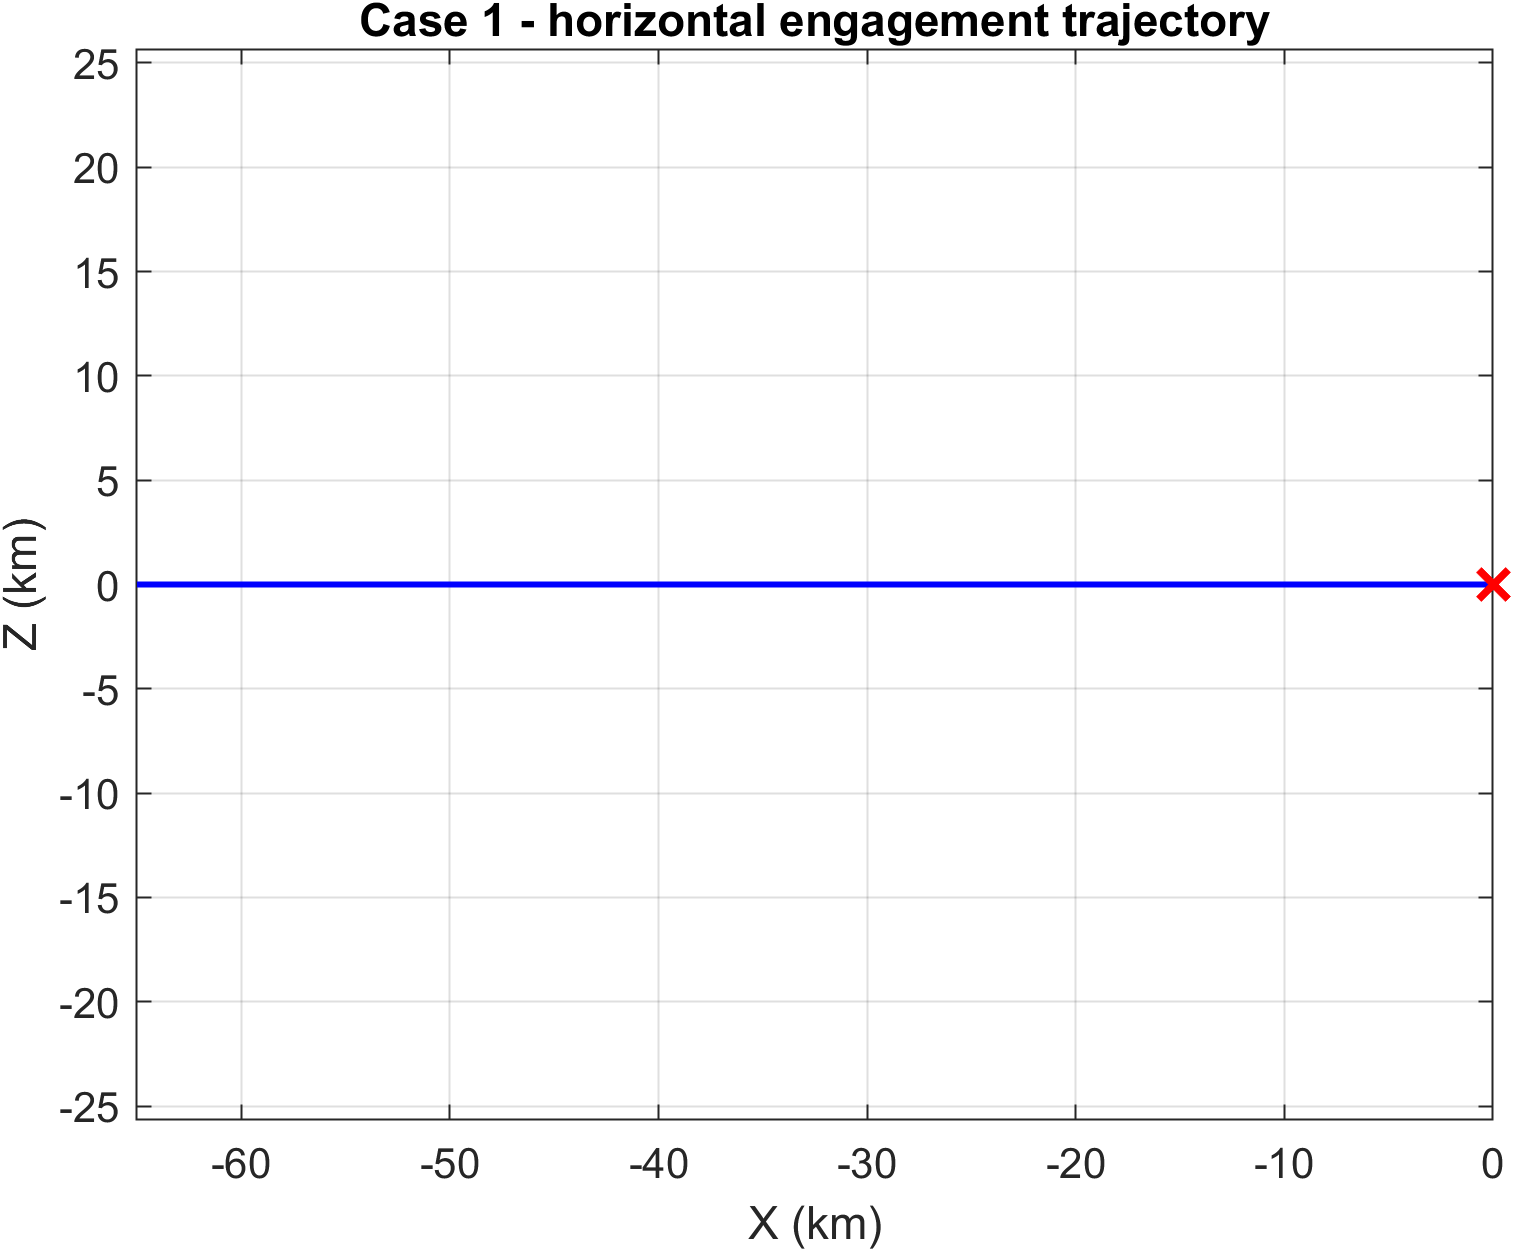
\includegraphics[width=0.78\textwidth]{figures/case1_engagement_trajectory.png}
\caption{Case 1 horizontal trajectory.}
\end{figure}

\begin{figure}[H]
\centering
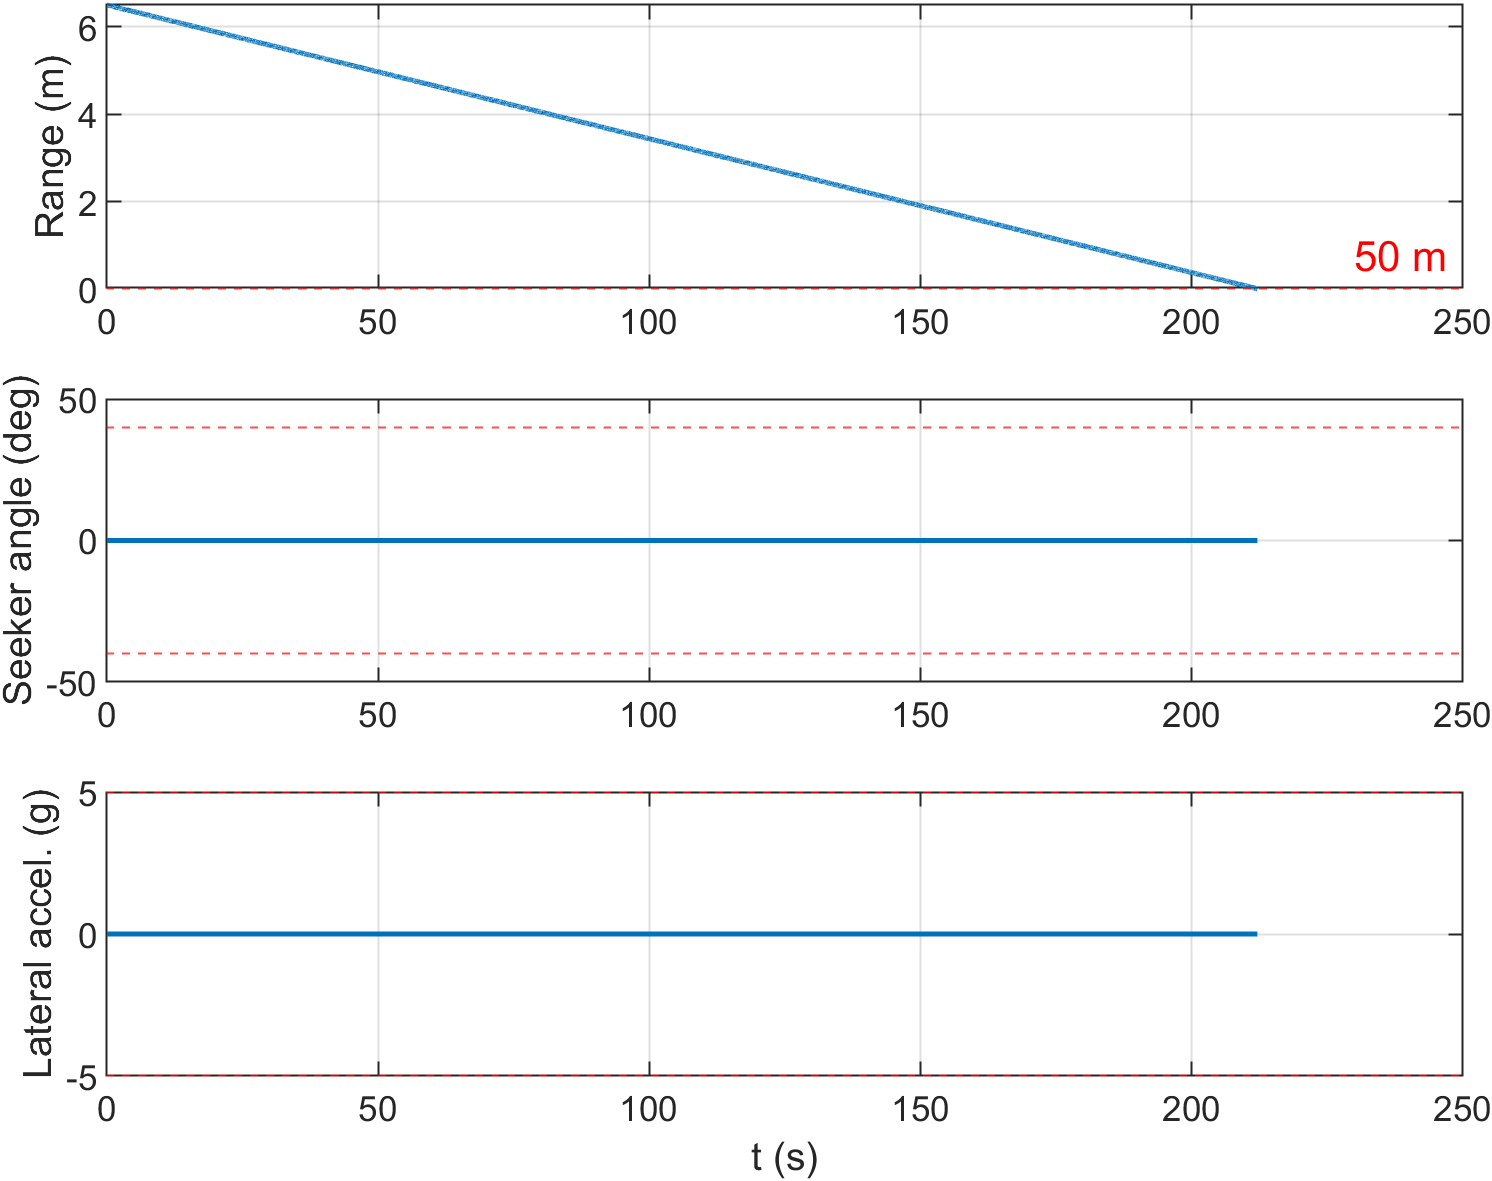
\includegraphics[width=0.92\textwidth]{figures/case1_engagement_history.png}
\caption{Case 1 range, seeker angle, and lateral acceleration.}
\end{figure}

\begin{figure}[H]
\centering
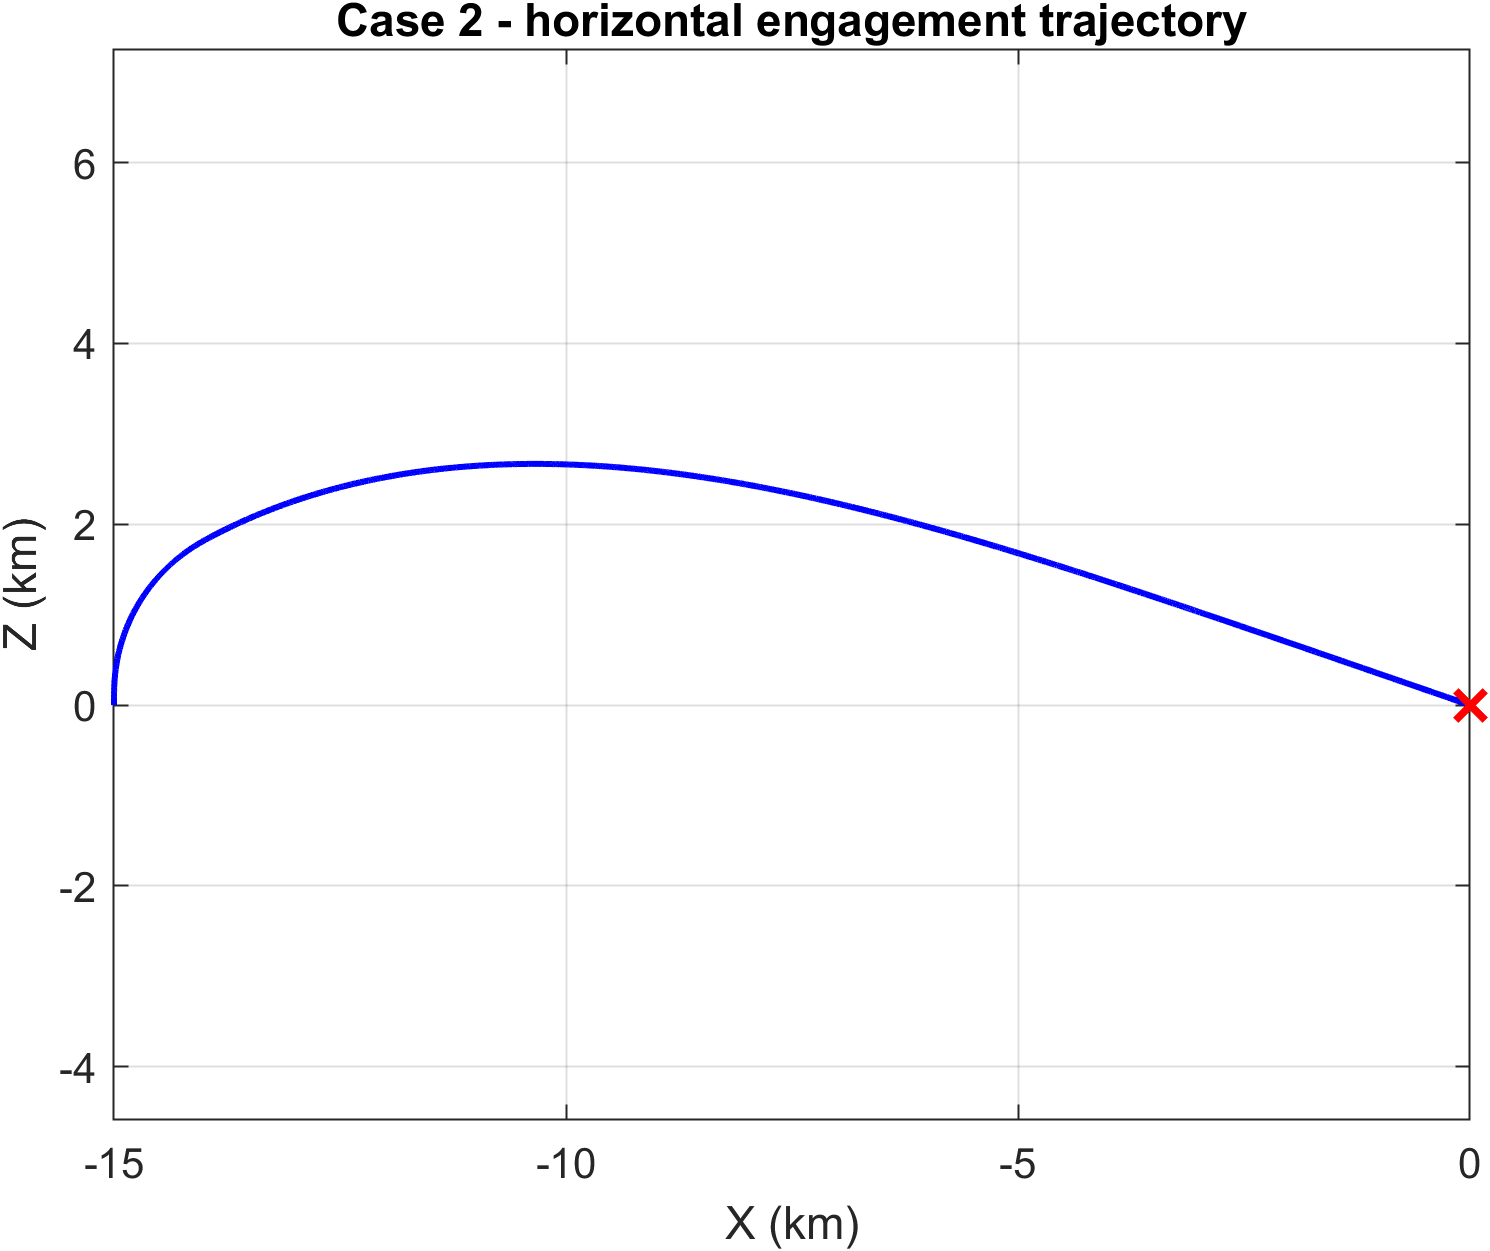
\includegraphics[width=0.78\textwidth]{figures/case2_engagement_trajectory.png}
\caption{Case 2 horizontal trajectory.}
\end{figure}

\begin{figure}[H]
\centering
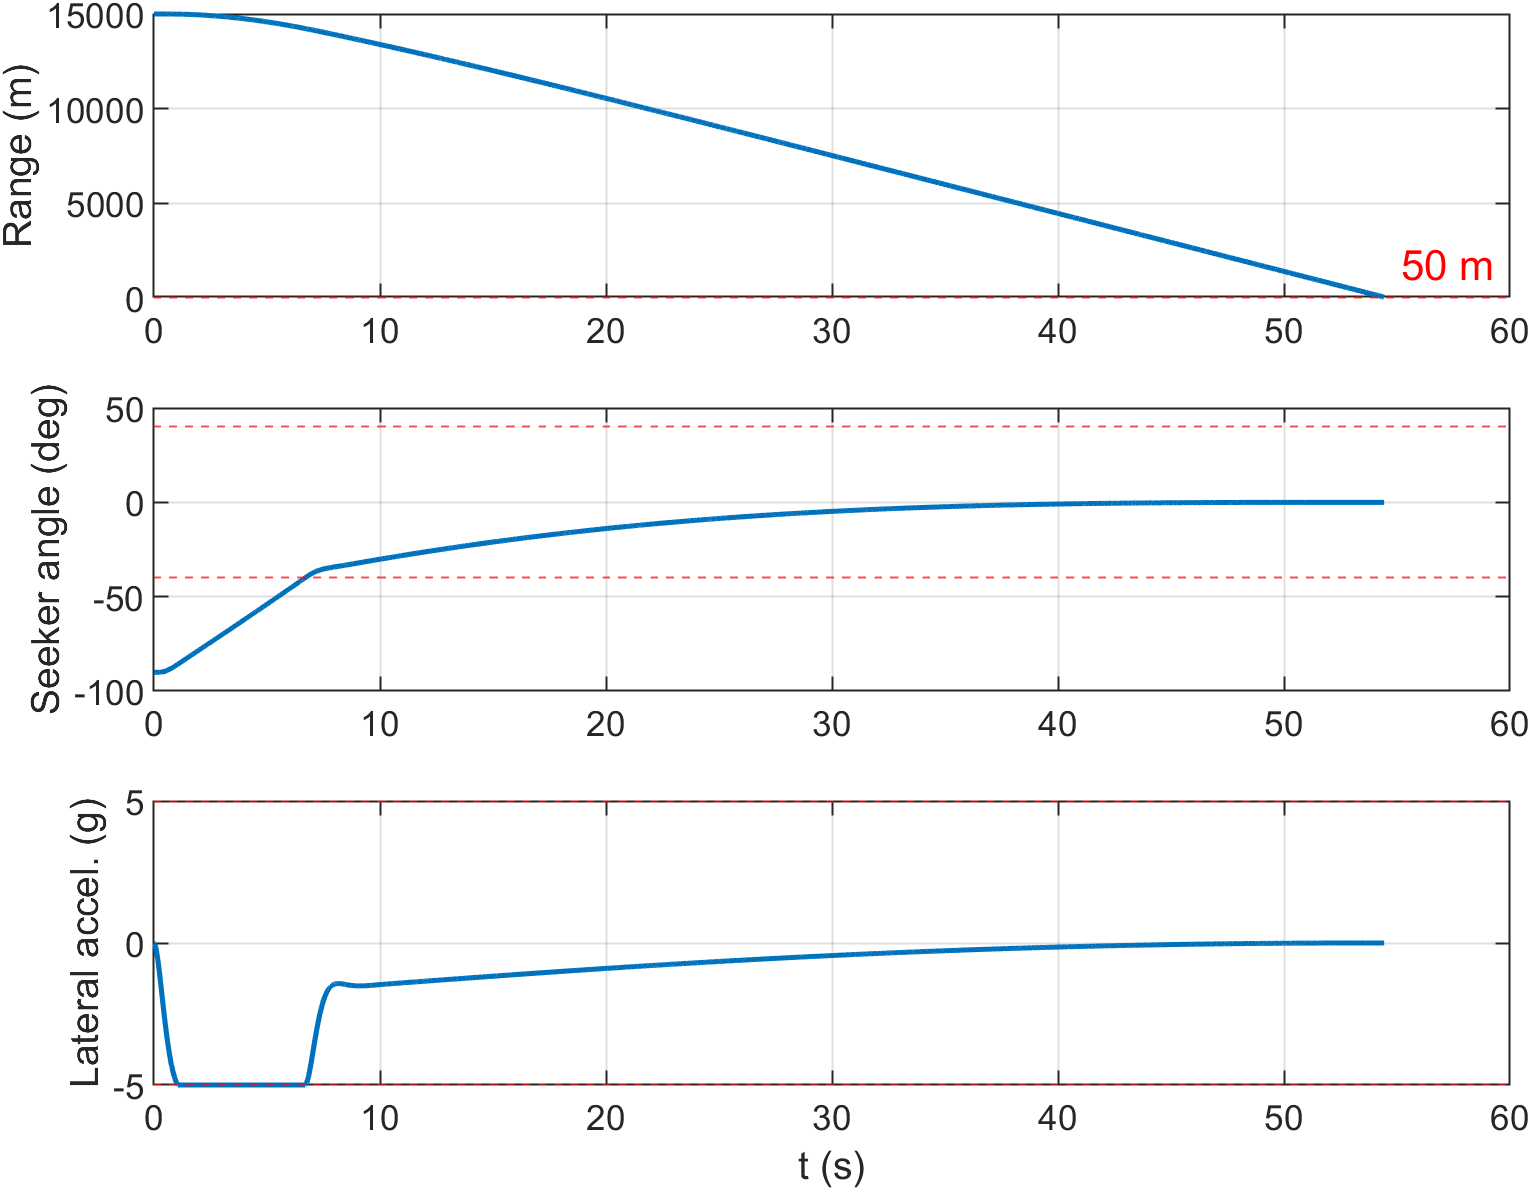
\includegraphics[width=0.92\textwidth]{figures/case2_engagement_history.png}
\caption{Case 2 range, seeker angle, and lateral acceleration.}
\end{figure}

Both cases satisfy the \(50~\text{m}\) miss-distance criterion. Case 1 is nearly collinear, so it requires almost no lateral acceleration. Case 2 uses the full \(5g\) limit during the initial turn, which is consistent with the harder \(90^\circ\) launch geometry.
